\documentclass[margin=10pt]{standalone}

\usepackage{tikz}

\usetikzlibrary{decorations.pathreplacing,arrows,shapes,positioning,shadows,calc}

\begin{document}

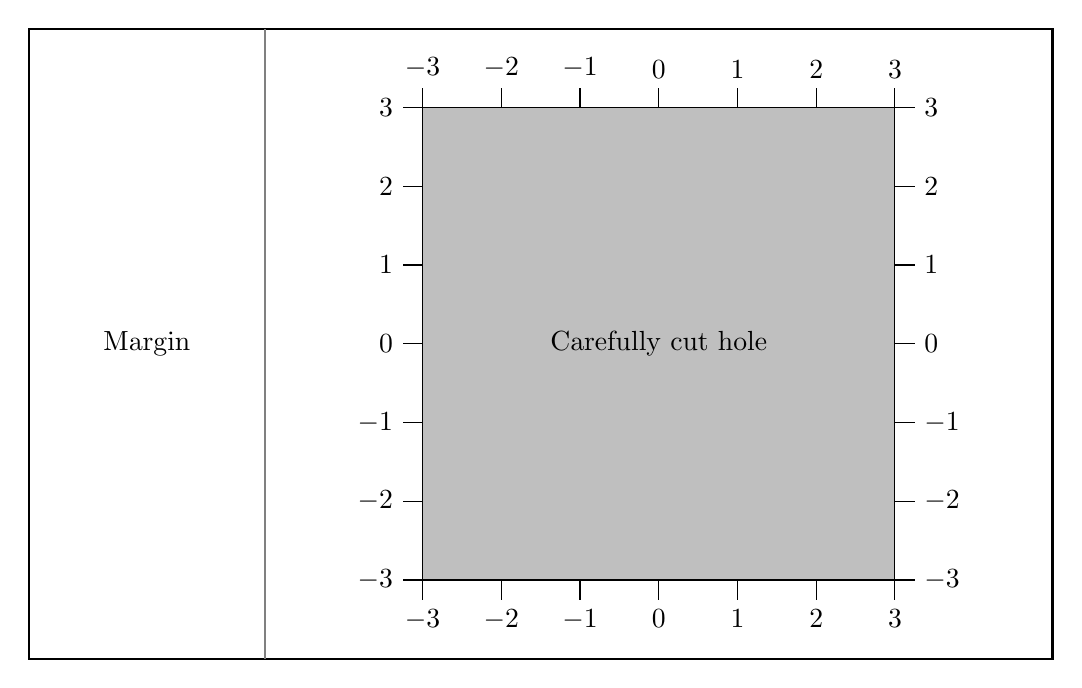
\begin{tikzpicture}
	\draw[thick] (0,0) rectangle (13,8);
	
	\draw[gray] (3,0) -- (3,8);
	\draw (1.5,4) node[anchor=center] {Margin};
	
	\draw[fill=lightgray] (5,1) rectangle (11,7);
	\draw (8,4) node[anchor=center] {Carefully cut hole};
	
	\draw (5,1) -- ++ (0,-0.25) node[anchor=north] {$-3$};
	\draw (6,1) -- ++ (0,-0.25) node[anchor=north] {$-2$};
	\draw (7,1) -- ++ (0,-0.25) node[anchor=north] {$-1$};
	\draw (8,1) -- ++ (0,-0.25) node[anchor=north] {$0$};
	\draw (9,1) -- ++ (0,-0.25) node[anchor=north] {$1$};
	\draw (10,1) -- ++ (0,-0.25) node[anchor=north] {$2$};
	\draw (11,1) -- ++ (0,-0.25) node[anchor=north] {$3$};

	\draw (5,7) -- ++ (0,0.25) node[anchor=south] {$-3$};
	\draw (6,7) -- ++ (0,0.25) node[anchor=south] {$-2$};
	\draw (7,7) -- ++ (0,0.25) node[anchor=south] {$-1$};
	\draw (8,7) -- ++ (0,0.25) node[anchor=south] {$0$};
	\draw (9,7) -- ++ (0,0.25) node[anchor=south] {$1$};
	\draw (10,7) -- ++ (0,0.25) node[anchor=south] {$2$};
	\draw (11,7) -- ++ (0,0.25) node[anchor=south] {$3$};
	
	\draw (5,1) -- ++ (-0.25,0) node[anchor=east] {$-3$};
	\draw (5,2) -- ++ (-0.25,0) node[anchor=east] {$-2$};
	\draw (5,3) -- ++ (-0.25,0) node[anchor=east] {$-1$};
	\draw (5,4) -- ++ (-0.25,0) node[anchor=east] {$0$};
	\draw (5,5) -- ++ (-0.25,0) node[anchor=east] {$1$};
	\draw (5,6) -- ++ (-0.25,0) node[anchor=east] {$2$};
	\draw (5,7) -- ++ (-0.25,0) node[anchor=east] {$3$};

	\draw (11,1) -- ++ (0.25,0) node[anchor=west] {$-3$};
	\draw (11,2) -- ++ (0.25,0) node[anchor=west] {$-2$};
	\draw (11,3) -- ++ (0.25,0) node[anchor=west] {$-1$};
	\draw (11,4) -- ++ (0.25,0) node[anchor=west] {$0$};
	\draw (11,5) -- ++ (0.25,0) node[anchor=west] {$1$};
	\draw (11,6) -- ++ (0.25,0) node[anchor=west] {$2$};
	\draw (11,7) -- ++ (0.25,0) node[anchor=west] {$3$};
\end{tikzpicture}

\end{document}